\documentclass[12pt,letterpaper]{report}
\usepackage[margin=1in]{geometry}
\usepackage{graphicx}
\usepackage{amsmath}
\usepackage[font=small,labelfont=bf]{caption}
\usepackage[justification=centering]{caption}
\usepackage{tikz}
\usepackage{circuitikz}
\usepackage{siunitx}
\usepackage{float}
\newlength \figwidth
\setlength \figwidth {0.75\linewidth}

\begin{document}

\title{E153 Laboratory Assignment \#6}
\author{Courtney Keeler and Stephen Pinto\\
Harvey Mudd College}
\date{November 20, 2013}
\maketitle

\section*{List of Materials}
\begin{itemize}
	\item Tektronix 2212 Oscilloscope
	\item Pomona 4550B (10X probe)
	\item Elenco LCM-1950 Multimeter
	\item 2N3904 transistor
	\item Standard resistors
	\item Standard capacitors
\end{itemize}

\section*{Purpose}
The purpose of this lab is to build a pre-designed common emitter amplifier and compare the actual performance to the simulated performance. The purpose is also to examine the effects of loading on the CE amplifier circuit by cascading the amplifier with a simple emitter follower.

\section*{Common Emitter Amplifier}
\subsection*{Procedure}

\begin{enumerate}
\item Measure the actual component values used in the CE design
\item Recalculate the gain and frequency response of the CE amplifier with the values from the previous step
\item Build the common emitter transistor amplifier designed in design project \#1
\item Compare the actual gain and frequency response values with the simulated values
\item Tweak component values 
\end{enumerate}

\subsection*{Results}

Measured component values for common emitter amplifier:
\begin{itemize}
\item $R_C$ = 17.67 k$\Omega$
\item $R_1$ = 10.1 M$\Omega$
\item $R_2$ = 18.24 M$\Omega$
\item $R_{E1}$ = 550 $\Omega$
\item $R_{E2}$ = 4.58 k$\Omega$
\item $C_1$ = .339 + .342 = .681 $\mu$F
\item $C_2$ = 323.5 + 332.3 = 655.8 $\mu$F
\item $\beta$ = 231
\end{itemize}

%photo 297
%gain is 26.6

%when both emitter resistors are bypassed, the gain beccomes just over 200

\subsection*{Calculations}

%real resistor and capacitor values
We want to recalculate the expected gain using the actual component values:
$$
A_v = \frac{-\beta R_C}{r_{\pi}+(1+\beta)R_{E1}}.
$$
First we must calculate $I_B$ so that we can know the value of $r_{\pi}$:
$$
I_B = \frac{V_{th}-0.7}{R_{th}+(1+\beta)(R_{E1}+R_{E2})},
$$
where
$$
V_{th} = \frac{R_2}{R_1+R_2}V_{cc} = 12.87 \text{ V}\, \text{ and } \, 
R_{th} = R_1||R_2 = 6.5 \text{ M}\Omega.
$$
We can plug all of this in to find:
$$
A_v = -28.34.
$$

\subsection*{Physical Implementation \& Analysis}

\begin{figure}[H]
\centering
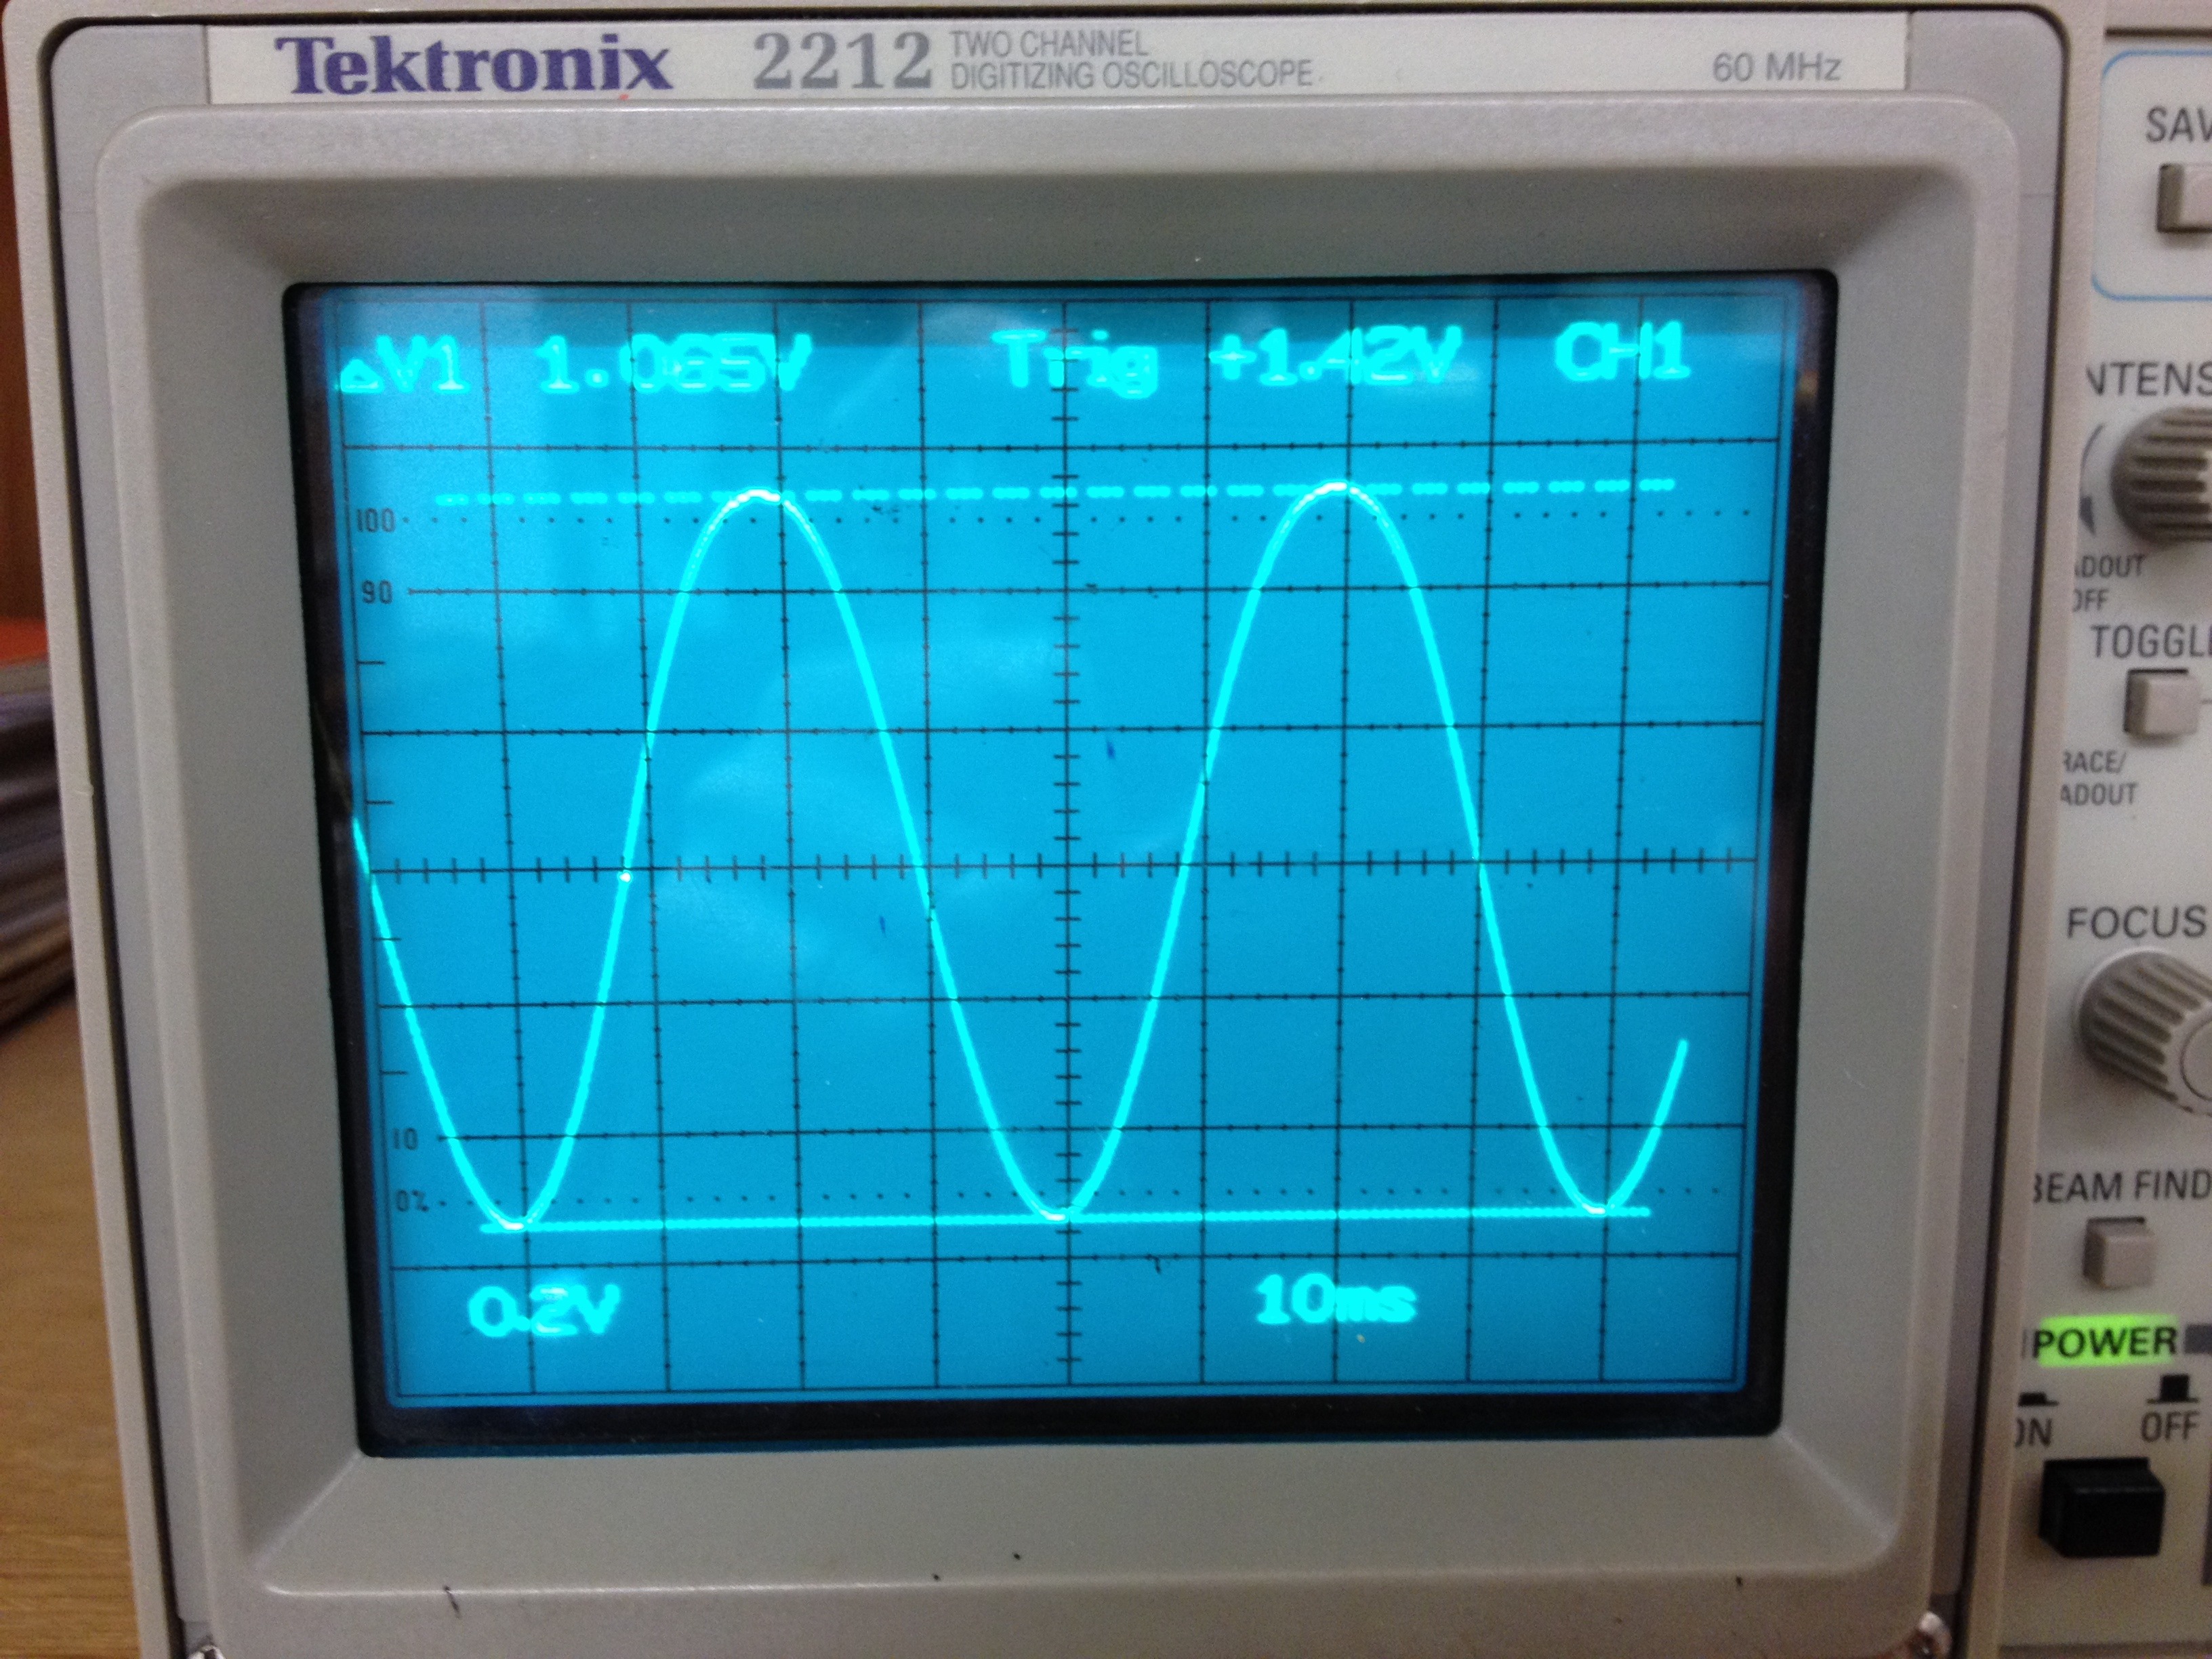
\includegraphics[width=\figwidth, keepaspectratio=true]{lab6_images/simple_output.jpg}
\caption{Output from Common Emitter Amplifier with input of 400  $mV_{pp}$.}
\label{fig:simple_output}
\end{figure}

Figure \ref{fig:simple_output} shows the 10.65 $V_{pp}$ output from the common emitter amplifier with an input of 400 $mV_{pp}$ - making the actual gain -27. While the magnitude of this measured gain is 6\% lower than expected, at least the measured gain is within the design specifications of $-25 \pm 10\%$. The reasons for this discrepancy could be 

\section*{Emitter Follower}
\subsection*{Procedure}

\begin{enumerate}
\item Add a simple emitter follower to the CE amplifier from the previous section
\item Calculate the theoretical voltage gain reduction caused by the added loading
\item Measure the actual voltage gain
\item Measure the output impedance for small signals
\item Measure the 
\end{enumerate}

\subsection*{Calculations}

Without the emitter follower attached, the output amplitude, as shown in Figure \ref{fig:simple_output}, is 10.65 $V_{pp}$. Since the emitter follower has some non-infinite input impedance, the output signal from the common emitter amplifier should have a reduced amplitude due to loading. This expected reduction is summarized by the following (where CEA stands for Common Emitter Amplifier and EF for Emitter Follower)
$$
V_{CEA,closed} = V_{CEA,open}\frac{R_{in,EF}}{R_{out,CEA}+R_{in,EF}},
$$
where $R_{in,EF}$ is approximately $(1+\beta)R_E$ since $r_{\pi,EF} \ll (1+\beta)R_E$ and $R_{out,CEA} = R_C$ . Thus
$$
V_{CEA,closed} = 10.65 \frac{(1+243)982}{17670+(1+243)982} = 9.87 V.
$$


\subsection*{Results}

\begin{figure}[H]
\centering
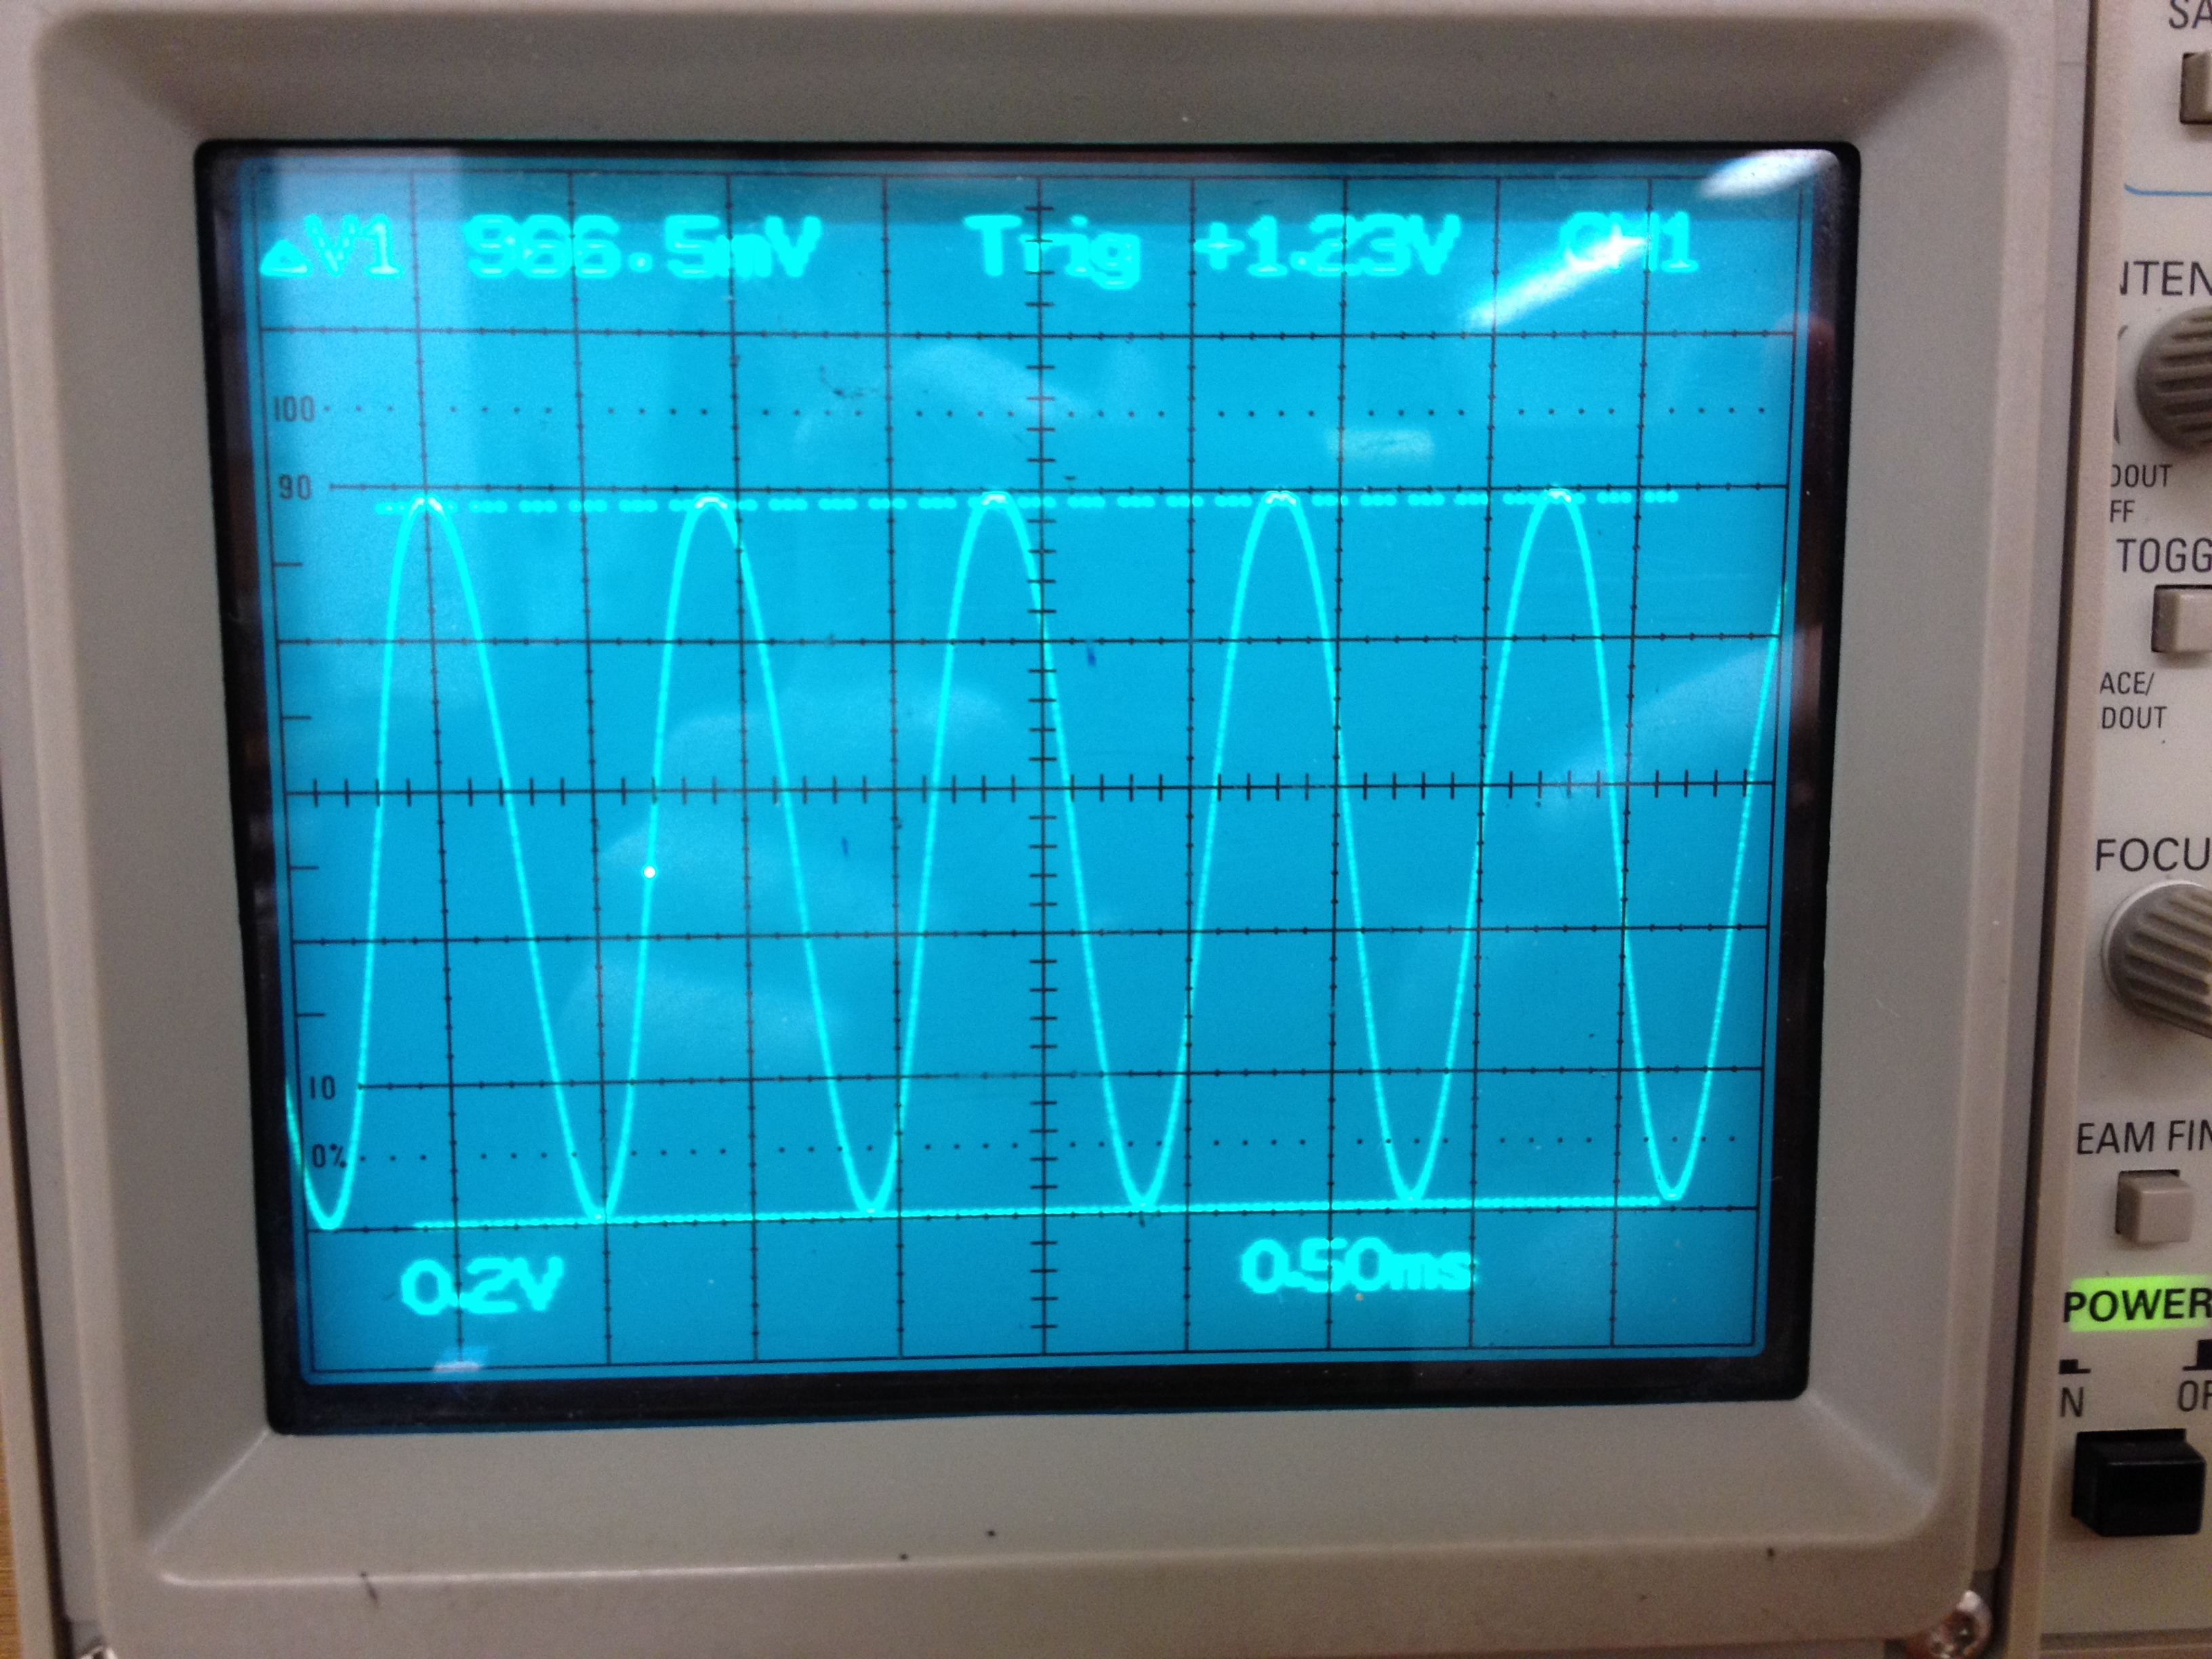
\includegraphics[width=\figwidth, keepaspectratio=true]{lab6_images/loading_output.jpg}
\caption{Output from Common Emitter Amplifier with input of 400 $mV_{pp}$ and emitter follower loading.}
\label{fig:loading_output}
\end{figure}

The measured component values for the emitter follower are $R_{E}$ = 982 $\Omega$ and $\beta$ = 243. Thus the expected voltage after the Common Emitter Amplifier is

$$
V_{CEA,closed} = 10.65 \frac{(1+243)982}{17670+(1+243)982} = 9.87 V.
$$

As shown in Figure \ref{fig:loading_output}, the measured voltage at that point was $V_{CEA,closed}$ = 9.67 $V_{pp}$, 2\% below the expected output.

Measured input amplitude at which output became non-linear: 500 m$\text{V}_{pp}$.
%becomes non-linear very quickly: 500mVpp (reaches saturation)


%small signal output impedance derivation:

\subsection*{Analysis}

We expect to see a drop in voltage gain when the emitter follower is added because it adds a load to the output of the common emitter amplifier. The larger this load is, the smaller the drop is signal gain. We see a drop from 10.6 V out to 9.6 V out, which corresponds well to the calculated expected value. The discrepancy of 0.2 V can be attributed to inaccuracy in measurements.

The output saturates very quickly when the input amplitude is increased to find the start of the non-linear response region. The emitter follower is responsible for this because it saturates high very quickly due to the fact that there is no resistor on the collector branch, which means the Q point voltage is high and already closer to the $V_{cc}$ value.
%emitter follower is saturating high because there is no Rc, so the Q point is high in voltage and is saturating at 20 V

\section*{Conclusion}

In conclusion, this lab has shown that 
. The purposes of the lab, which was to build a pre-designed common emitter amplifier and compare the actual performance to the simulated performance, as well as  examine the effects of loading on the CE amplifier circuit, were met.

\end{document}

%photo 297: output of entire CE circuit, shows gain at 25 Hz
%photo 298: voltage after stage 1
%photo 299: voltage after emitter follower (it's been shifter down by 0.7!)

%\begin{table}[ht]
%\caption{Voltage across each "diode"} % title of Table
%\centering 
%    \begin{tabular}{| c | c |} 
%    \hline
%    $V_{\text{BC}}$ & 0.711 V \\
%    $V_{\text{BE}}$ & 0.717 V \\
%    \hline
%    \end{tabular}
%    \label{table:section_1}
%\end{table}
